\section{Анализ графиков}

Ниже показаны результаты выполнения алгоритма Дейкстры с использованием 3-кучи и 15-кучи на графах, варьирующихся по количеству вершин и рёбер. Эти эксперименты позволяют оценить влияние структуры кучи на производительность алгоритма при изменении различных параметров графа.

\begin{figure}[H]
    \centering
    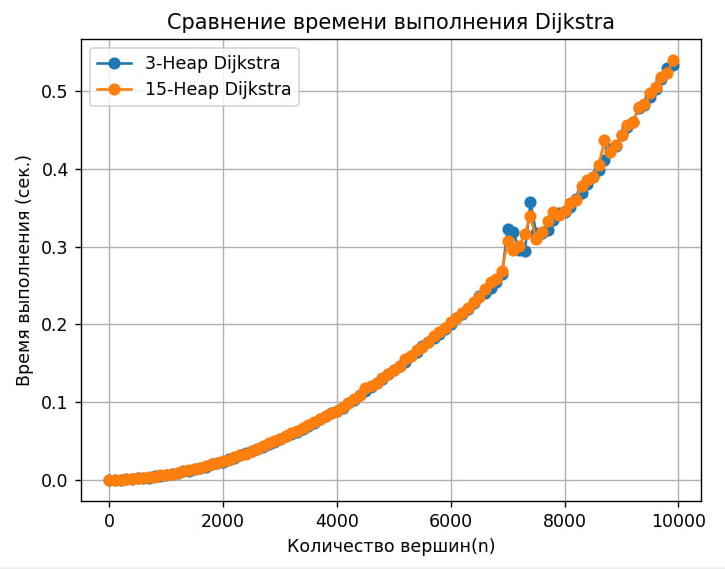
\includegraphics[width=0.8\linewidth]{picture/vertices.png}
    \caption{Сравнение времени выполнения в зависимости от количества вершин}
    \label{fig:vertices}
\end{figure}

На графике~\ref{fig:vertices} представлена зависимость времени выполнения от количества вершин \( n \). Здесь видно, что использование как 3-кучи, так и 15-кучи приводит к схожим результатам. Различия в скорости выполнения становятся заметны только при больших значениях \( n \), при этом 15-куча начинает слегка уступать 3-куче по скорости выполнения. Это может быть связано с тем, что при увеличении арности увеличивается количество операций управления в более крупных кучах.

\begin{figure}[H]
    \centering
    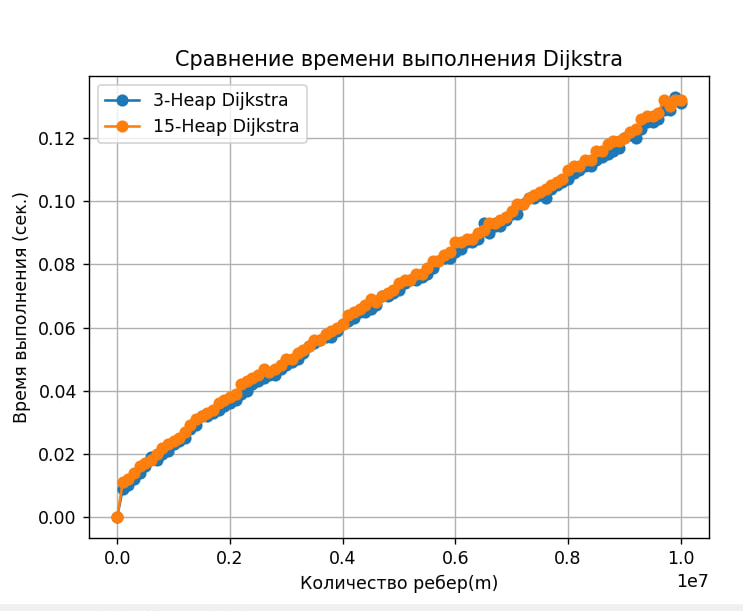
\includegraphics[width=0.8\linewidth]{picture/edges.png}
    \caption{Сравнение времени выполнения в зависимости от количества рёбер}
    \label{fig:edges}
\end{figure}

На графике ~\ref{fig:edges} представлена зависимость времени выполнения от количества рёбер \( m \). В этом случае время выполнения алгоритма также линейно возрастает с увеличением \( m \), и различия между 3-кучей и 15-кучей остаются минимальными. Однако, как и в случае с увеличением вершин, можно заметить, что 15-куча начинает показывать слегка большее время выполнения на больших значениях \( m \). Это связано с тем, что на больших графах операции в 15-куче могут требовать больше времени для поддержания структуры кучи при добавлении и удалении элементов.


\section*{Возможные причины отклонений:}
На графиках также можно заметить незначительные отклонения, которые могут быть обусловлены фоновыми процессами операционной системы, влиянием кэширования и доступом к оперативной памяти. Эти факторы могли вызвать незначительные колебания во времени выполнения, особенно при многократном запуске алгоритма на больших графах.
